%!TEX root = thesis.tex

In this thesis we will introduce the notion of \emph{ad hoc interfaces} or AHIs.

Being \emph{ad hoc} generelly means something made for a specific task or creating meaning in changing contexts.
The word itself originates from the Latin language and literally means \emph{for this} (situation). 
In modern english the two word combination is regarded as a single word and the Oxford Dictionary\footnote{http://oxforddictionaries.com/definition/english/ad-hoc} defines it as

\begin{quotation}
\textbf{Ad hoc}  /ad 'h\textturnscripta k/

created or done for a particular purpose as necessary
\end{quotation}

The word is used in many different fields and context.
For example, In society committees a formed on an ad hoc basis to deal with specific tasks, investigations or analyses.

In computer science wireless networking can be of an ad hoc nature, which means that that the network is not dependent on a preexisting infrastructure.
Wireless ad hoc networks are highly dynamic and all participating nodes in the network graph are more or less doing routing for each other.
This makes the network adaptive to changing contexts, which is an important element of ubiquitous computing.

In general a user works with a computer in an ad hoc manner.
General purpose computers are very good at supporting ad hoc activities with their multitasking capabilities.
Applications are used when needed and maybe even used in connection with each other.
Windows are opened, closed and arranged as needed to support different use cases.

So, ad hoc is a prevalent characteristic within many activities and contexts.
Next we will give our own definition of being ad hoc when applied to the field of user interfaces and also compare this to other elements of \todo{computer science}.

\section{Defining ad hoc interfaces} 
We define ad hoc interfaces as 

\begin{quotation}\label{adhoc:definition}
\emph{physical interfaces that can be \todo{created} or accessed on} 

\emph{demand for a particular purpose in mind. }
\end{quotation}

In this sense there is a degree of temporality embedded in the definition, in that the interaction is somewhat impromptu and the purpose is non-continuing.
The interface can be accessed when needed and when the interaction and purpose has ended it ``disappears'' again.
This makes good sense in the digital realm as pixels on a screen can easily be controlled and abstracted to bring attention to different tasks.
The questions is, how do we apply these ad hoc elements or characteristics to physical interfaces.
The physical world comes with many constraints compared to the digital as we are limited by the characteristics of the materials we interact with and the general laws of physics.
We can't just magically make physical objects appear and disappear which is possible, and easy, to do on a digital display.

We see two overall approaches to creating physical interfaces with ad hoc capabilities \todo{Stefan sees two ways while writing this ;-)}.
\begin{itemize}
	\item{Through invisible interfaces embedded into the physical environment}
	\item{Using shape change as the construction mechanism}
\end{itemize}

The two approaches does not exclude each other as they could surely be combined while still living up to our definition.
In the following we will elaborate on each approach separately.

\subsubsection{Embedding invisible interfaces into the physical environment}

In this case an existing element of the environment will contain the interface.
An element can be both a physical object, for example walls, furniture, devices etc, and also ambient air \todo{there is a better word for this}.
The perceived action possibilities are constrained by the affordances of the object. 
The input and output possibilities depend on the materiality of the physical object.
A variety of sensors can be used for input and actuators for output.

In \autoref{ch:textile-touch} we explore this approach.

\subsubsection{Using shape change as the construction mechanism}

In this case an objects shape changing capabilities lets it shift or morph into an particular interface.
Affordances are here dictated by the perceived action possibilities of the particular end-shape.
Again, sensors and actuators can be embedded for input and output control.
``No longer does form follow function, form becomes function''

In \autoref{ch:jamming} we explore this approach.

\todo{But what can we do} 
\begin{verbatim}
create interface: shape-change tilgange
create i bogstavelig forstand: bare paint
access interface: textile-touch

introducerer muligheden for baade space- og time multiplexing
\end{verbatim}

Let's first have a look at some existing products and projects which we have found that exhibit ad hoc characteristics. \todo{\ensuremath{\leftarrow} overgang til naeste subsektion}

\subsection{Products with ad hoc characteristics}
Ad hoc characteristics in interfaces are not some novel invention and they an be found in several existing products.
A simple example would be The Clapper\footnote{http://en.wikipedia.org/wiki/The\_Clapper} (figure~\ref{ch:adhoc:theclapper}) from the mid eighties, an electrical switch reacting to sounds in a specific frequency, tuned to claps, to turn a switch on and off respectively.
Here the interface is pervasive in the nearby environment and one interacts with it when needed after which it ``disappears'' again.

\begin{figure}[hb]
	\centering
  		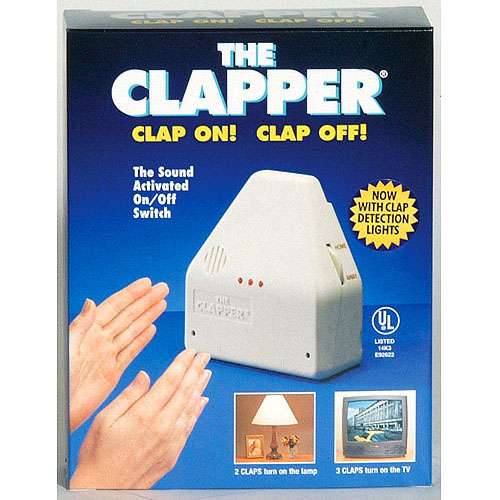
\includegraphics[width=1in]{figures/theclapper}
	\caption[The Clapper, a sound activated electronic switch.]
   {The Clapper, a sound activated electronic switch.}
   \label{ch:adhoc:theclapper}
\end{figure}

Another example is the conceptual and somewhat futuristic product ShapePhone (figure~\ref{fig:ch:jamming:jui-phone}) based on particle jamming, which will also be addressed in \autoref{ch:jamming}.
ShapePhone is generic shape changing product which changes it behaviour based on its physical form.
For example, in its base form it is a phone but when wrapped around a wrist it could serve as a watch and when folded in some other way it could be a game controller.
So, the different interfaces are created on demand by the user and have very different purposes of use depending on the form of the interface.

In a masters course in 2011 called Innovation Project \cite{innoproj2011, beomotionreportstefan, beomotionreporttore}  we, the authors, designed and implemented a dynamic shape shifting wall module with the ability to change its surface structure for acoustic regulation, i.e. diffusion, absorption and reflection for optimal conditions.
On top of that the module had illuminating features so that different areas could light up and serve as an aesthetic lighting for the atmosphere of the room.
The idea for the module was to retain the aesthetics of existing surroundings, so the module was not in use, the module would be `invisible' and flat like the wall.  
We envisioned two scenarios of use for the wall.
One where context awareness was the primary driver which meant that everything (acoustic and lighting conditions) would be automatically sensed and the wall module would modify itself accordingly and shift from flat to active.
In the other scenario the user would, to a higher degree, be in control.
The user could actively create deformations on the surface for aesthetic purposes and also control illuminated areas by interacting with the wall surface, see \ref{fig:ch:adhoc:beomotion}.
In this scenario the interface was shaped and created by the user for the specific situation, i.e. current acoustic and lightning conditions, as well as the desired aesthetic expression. 

\todo{afslut afrunding} And of course, also the inherent ad hoc nature of the way we interact with personal computers as mentioned in the introduction of this chapter.
\blank
\todo{2-3 flere eksempler \dots} 

\begin{figure}
	\centering
	\begin{subfigure}{.46\textwidth}
		\centering
		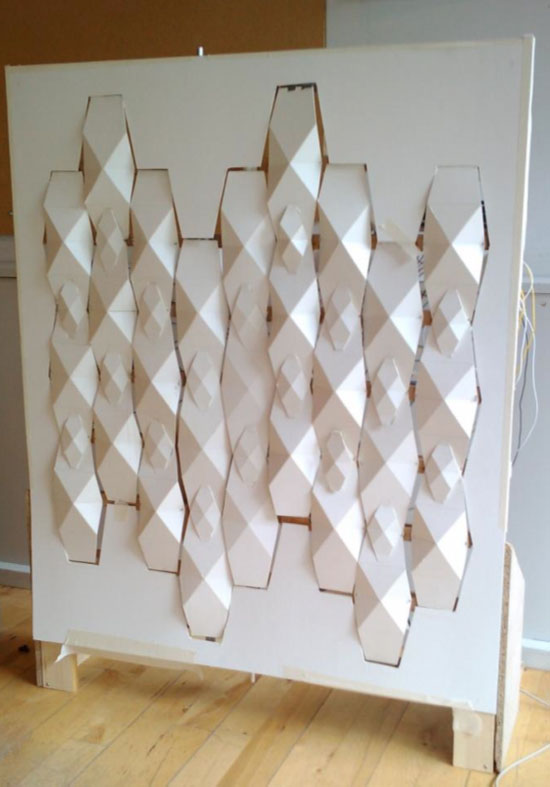
\includegraphics[width=.9\linewidth]{figures/beomotion/prototype}
		\caption{Interactive prototype}
	\end{subfigure}%
	\begin{subfigure}{.54\textwidth}
		\centering
		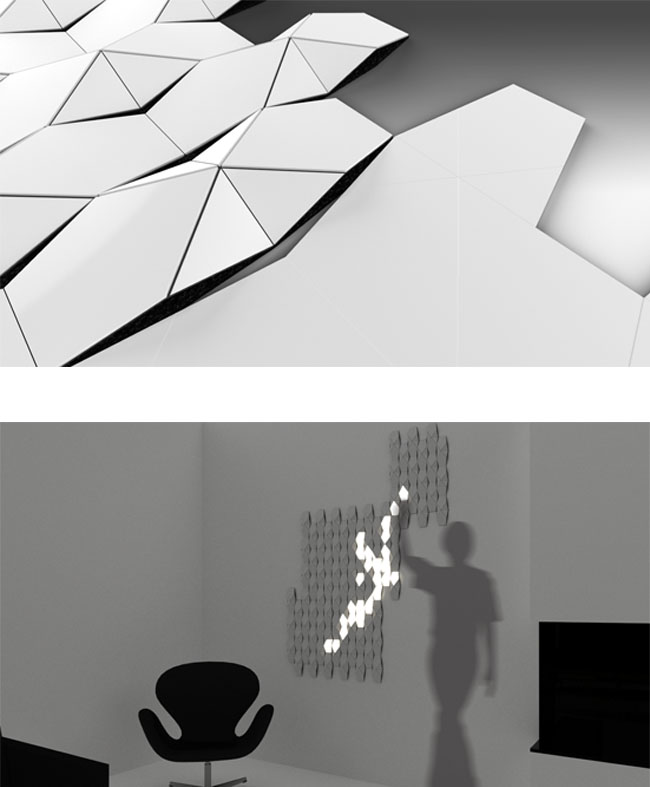
\includegraphics[width=.9\linewidth]{figures/beomotion/concepts}
		\caption{Concept illustrations}
	\end{subfigure}
	\caption{BeoMotion product design, Innovation Project, Aarhus University 2011}
	\label{fig:ch:adhoc:beomotion}
\end{figure}

\subsection{Relationship with other fields} 
% CAC comparison
It might seem that AHI overlaps with the concept of Context Aware Computing in that they both have a focus on environmental context.
In context aware computing a system attempts to derive, through a variety of cues, what the current context of use is and as a result it adapts its behaviour \citep[chap. 8]{krumm2009ubiquitous}. 
In this way it is the system itself that takes action autonomously and the user continues on outside of the control loop. \todo{rephrase??}
Exactly the topic of control is one of the points where context aware systems have received criticism \cite{erickson2002some}, \citep[chap. 8]{krumm2009ubiquitous}.
The criticism has to do with a systems ability to make inference based on the analysis of quantitative contextual information available, something that can be quite difficult to do for a computer as contextual information is often subtle and implicit.
\todo{This is not supposed to be a critique of context aware systems as they surely have their legitimacy and offer a lot of convenience.}
\todo{An AHI can have CAC elements} 

Where context aware systems put the user out of the control loop AHIs do not.
In AHIs the user is the initiator of action.

It actually makes no sense to compare them directly as they cannot be juxtaposed.
They are both elements or characteristics of a system and one does not exclude the other as a part of a system.
It would seem quite natural to have an ad hoc system that also incorporates some context aware computing elements, for example \todo{give a good example} 
\blank
% TUI comparison
Tangible user interfaces, or TUIs, do generally not exhibit ad hoc characteristics. \todo{det skal lige overvejes om det er helt sandt- NEJ}
They are mentioned here more for their nature of physical representation and their movement away from the standard GUI paradigm for human-computer interaction.
TUIs demonstrate a inherently tight coupling between digital information and the associated physical representation, for example tangible tokens representing a specific digital entity or mapping to a specific function or action.
There are numerous examples of these, for example, the ReacTable \cite{jorda2007reactable}, the Marble Answering Machine \todo{citation possible or link} to name a few.
Furthermore, because of this tight coupling the physical representations are often created only for the specific purpose and are of no use outside of the TUI context. \todo{er det at sk\ae re det over en kam??}

In contrast, ad hoc interfaces define a more loose coupling meaning that one physical object can serve several purposes. \todo{igen - ???}
This will be exemplified in \autoref{ch:textile-touch} where we prototype a general purpose ad hoc interface called textile touch, which can augment existing household objects by adding a digital layer.
\blank
\todo{and Augmented reality - While on the topic of adding a digital layer to the real-world environment we should also bring up the concept of Augmented Reality, or AR.}

\section{Discussion}

By giving an overview of related fields within HCI it is apparent that ad hoc interfaces relates in one way or another to other 

Opsumm\'er ad hoc
\begin{verbatim}
Ad hoc definiton
Some existing products exhibit ad hoc behaviour 
bringing together different aspects of various fields within HCI.

``fashioned from whatever is immediately available'' - may not quite be possible

Hvad aabner det op for.

\end{verbatim}